\chapter{Fundamentação Teórica}

O capítulo atual traz a fundamentação teórica necessária para o desenvolvimento deste trabalho, abrangendo a evolução da eletrônica e sistemas
embarcados veiculares, e a tecnologia de comunicação veículo-a-tudo (V2X). Serão introduzidos conceitos, definições e padrões tecnológicos, visando
construir uma base teórica sólida para desenvolver a simulação de tráfego e a subsequente análise dos benefícios da conectividade cooperativa na
segurança e eficiência do trafego urbano.

\section{Fundamentos da Eletrônica Veicular}

O mercado automotivo global na atualidade apresenta grande parte da competitividade e diferenciação entre os fabricantes quando o assunto é a eletrônica
integrada nos veículos. Um estudo publicado por \cite{ref:bccresearch} realizou a análise da cadeia de suprimentos e levantou dados sobre o crescimento
do mercado de eletrônicos na industria automotiva, onde os componentes eletrônicos já representam cerca de 30\% do valor valor total de fabricação de um
novo veículo movido a motores de combustão interna. Com a consolidação de novas tecnologias de conectividade, direção autônoma e eletrificação, projeta-se
que a eletrônica atinja uma participação de 50\% do valor total de fabricação de um veículo a combustão e chegando a 70\% em veículos elétricos (EVs).

Essa infraestrutura tecnológica é bem mais visível em veículos premium, que conseguem integrar mais de 100 ECUs interconectadas e distribuidas por todo o
veículo. Diversas redes diferentes como CAN, LIN, FlexRay e Ethernet são utilizadas para conectar os diversos subsistemas, assim como é mostrado na
Figura \ref{fig:vehicle_electronics_network}, onde múltiplas ECUs, sensores e atuadores se comunicam por meio de barramentos e redes de comunicação internas
ao veículo \cite{ref:leen2002}.

\begin{figure}[H]
    \centering
    \caption{Arquitetura típica de rede eletrônica veicular}
    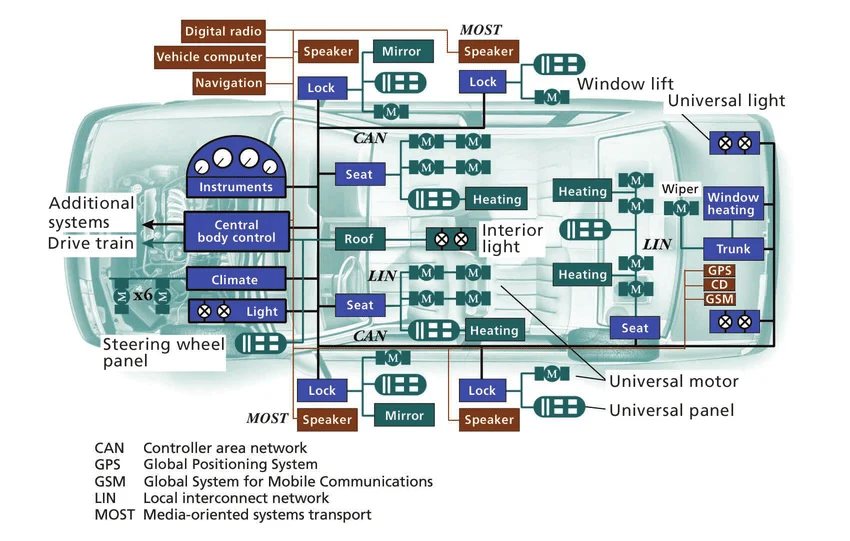
\includegraphics[width=0.85\linewidth]{figuras/vehicle_electronics_network.png}
    \label{fig:vehicle_electronics_network}
    \par\smallskip
    \small Fonte: Adaptado de Leen e Heffernan (2002).
\end{figure}

A Unidade de Controle Eletrônico (ECU) é o principal componente da arquitetura eletrônica moderna, operando de maneira dedicada funções específicas do
veículo. Tecnicalmente, as ECUs funcionam sob o modelo IPO (\textit{Input-Process-Output}), onde circuitos de entrada recebem sinais de sensores (como
temperatura e velocidade), microcontroladores processam os dados e executam algoritmos para tomada de decisão, e circuitos de saída utilizam os resultados
para controlar atuadores (como injetores de combustível e freios). De acordo com \cite{ref:munir2018}, os automóveis modernos evoluiram integrando uma centena
de processadores, que operam sob protocolos de comunicação em redes de alta velocidade para coordenar as funções do automóvel.

A integração dessas unidades de controle em uma arquitetura de rede complexa exige que o veículo seja tratado como um conjunto de sistemas distribuídos.
Funções criticas, como segurança ativa e controle de propulsão, dependem da comunicação eficiente entre varias ECUs através das redes do automóvel. Essa
grande quantidade de eletrônica integrada e uma crescente interdependência entre os subsistemas tornam o desenvolvimento, teste e validação de software
automotivo cada vez mais desafiadores, mas também traz a oportunidade do desenvolvimento de novas tecnologias e funcionalidades que permitem uma maior
consciência sobre o ambiente para uma melhor experiência de condução e segurança.

\section{Evolução da Eletrônica e Sistemas Embarcados}

A indústria automotiva tem passado por uma transformação significativa nas últimas décadas, tornando-se significativamente mais intensiva em sistemas
computacionais e softwares do que em sistemas mecânicos. Enquanto historicamente o desenvolvimento era dominado pela engenharia mecânica, hoje a parte
eletrônica e de software se tornaram o principal motor de inovação no setor automotivo. Essa transformação se iniciou por volta de 1970, com a introdução
das ECUs, que alterou as lógicas de comando das funcionalidades veículares.  

Veículos mais modernos apresentam um sistemas embarcados cada vez mais complexos, integrando uma variedade de radares, sensores e câmeras para aquisição de
dados. Como ilustrado na Figura \ref{fig:audi_a8}, o Audi A8 integra diversos componentes eletrônicos, que trabalham de forma conjunta, oferecendo ao motorista
funções avançadas de assistência à condução e segurança. Essa diversidade de dispositivos demonstra que a eletrônica se tornou algo fundamental para os veículos
atuais, trazendo tecnologias inovadoras ao mercado, como o sistema de direção autônoma e a conectividade veicular (V2X), que serão abordados posteriormente 
neste capítulo.

\begin{figure}[H]
    \centering
    \caption{Sensores e Câmeras do Audi A8}
    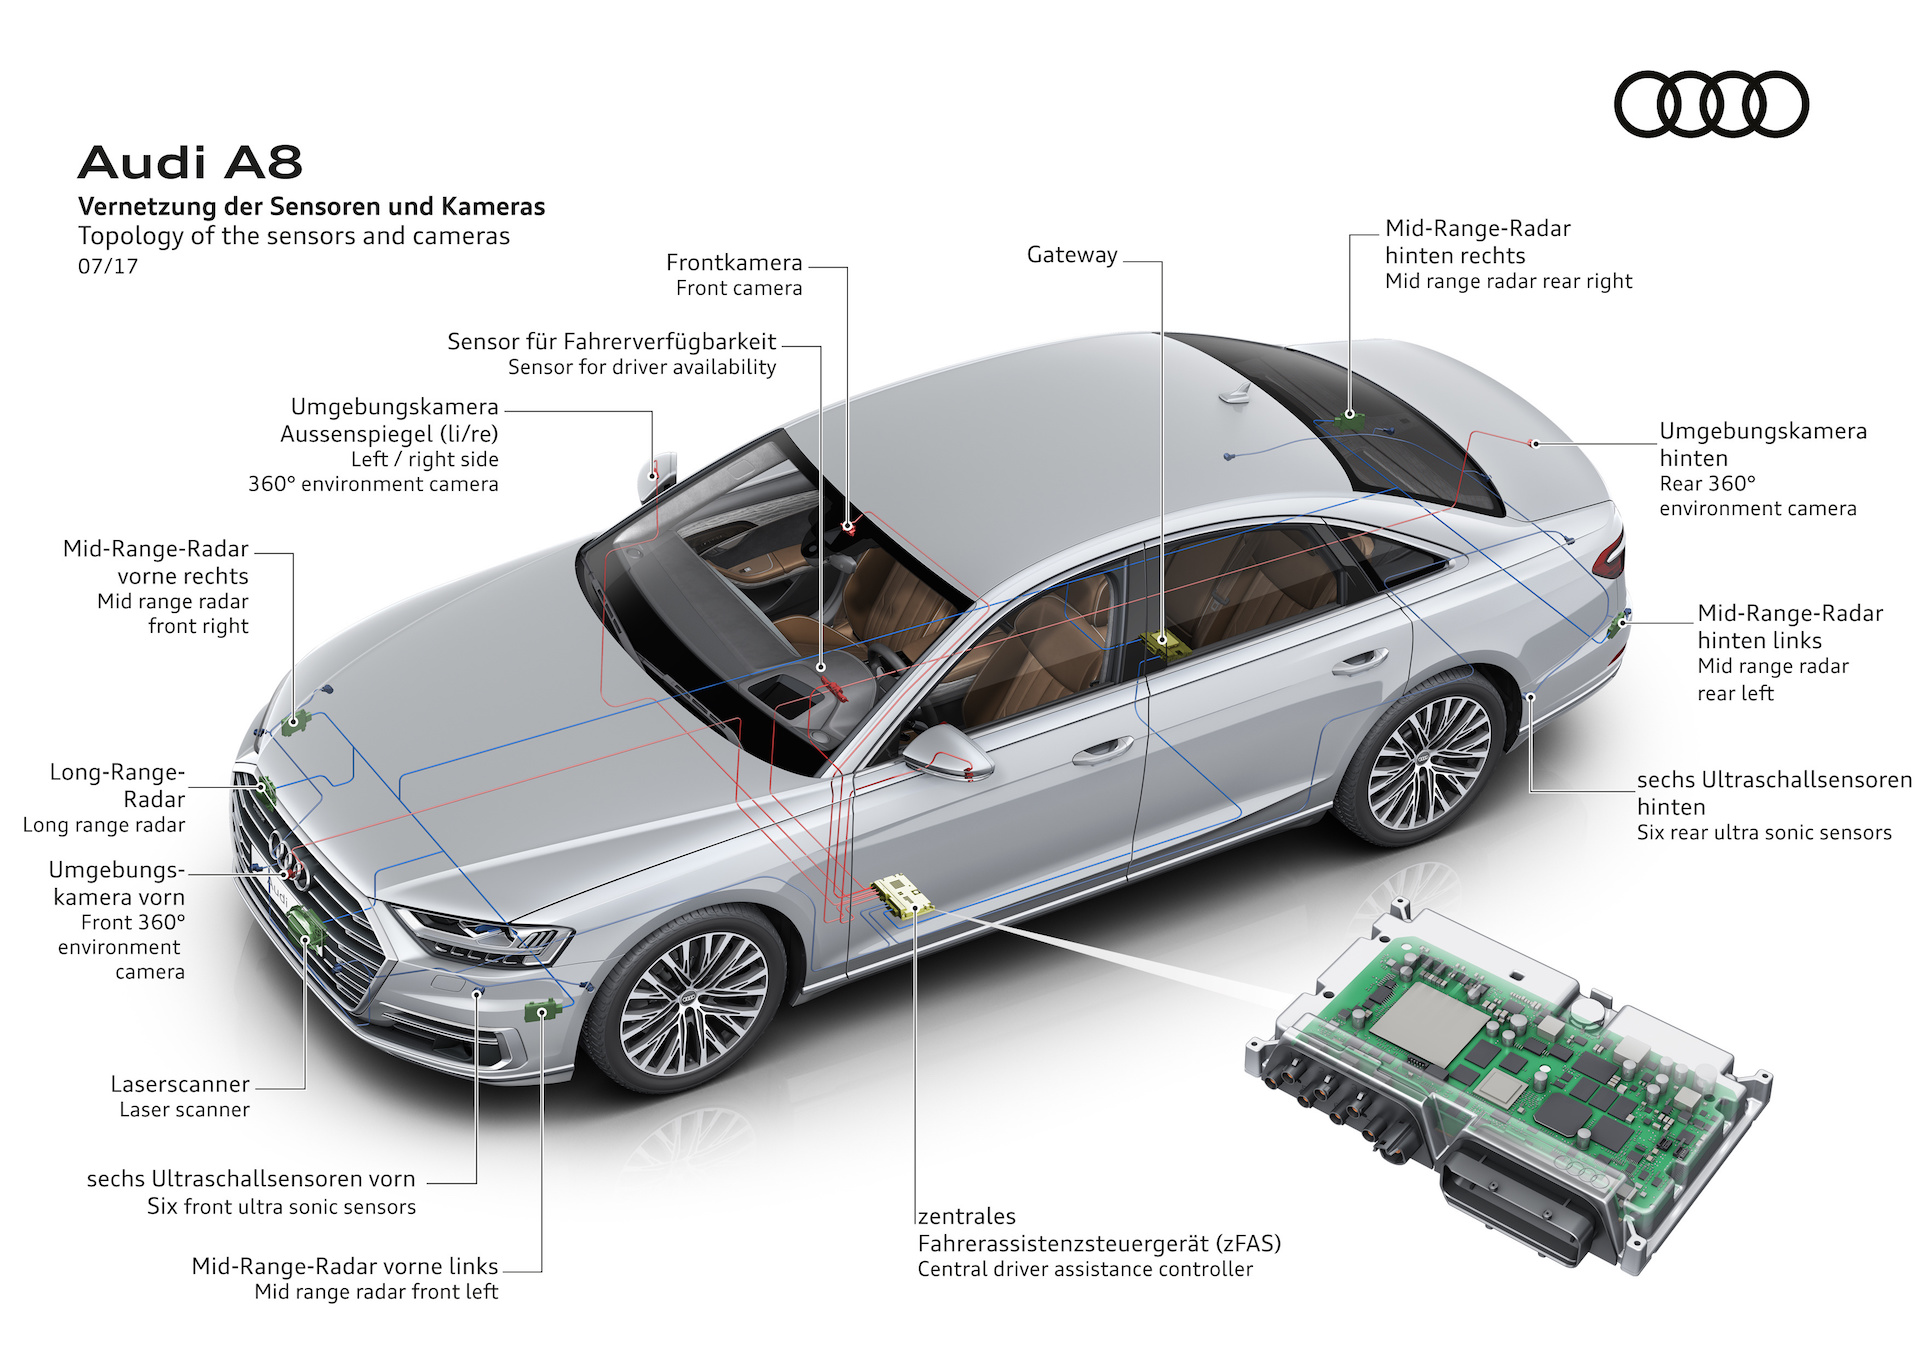
\includegraphics[width=0.85\linewidth]{figuras/audi_A8_sensors_and_cameras.jpg}
    \label{fig:audi_a8}
    \par\smallskip
    \small Fonte: Audi (2019).
\end{figure}

Como mencionado por \cite{ref:hodel} em seu trabalho sobre testes para software em sistemas embarcados automotivos, o setor está sendo impulsionado por
tecnologias como a eletrificação, a Internet das Coisas (IoT) e a automação, que além de necessitarem uma integração entre os subsistemas internos do veículo,
também necessitam uma comunicação com infraestruturas externas. Como esse nível de integração, fundamentamos a transição para um Sistema de Transporte Inteligente
(ITS), permitindo que o meio de transporte não sejam apenas limitados ao hardware instalado no veículo, mas também possam se comunicar com outros veículos e com
a infraestrutura urbana ao seu redor através da conectividade V2X.

\section{Tecnologia de Comunicação Veicular (V2X)}

A comunicação veicular consiste em uma tecnologia para troca de dados entre veículos e outros elementos do ambiente, aumentando a consciência situacional no
ambiente de tráfego, gestão operacional e a conveniência do usuário. A ideia principal desse tipo de comunicação é elevar o nível de segurança e eficiência do
transporte, permitindo que os automóveis recebam informações críticas que sistemas de bordo isolados não conseguem captar sozinhos, além de possibilitar
funcionalidades como a gestão de frotas em tempo real, monitoramento de condições de tráfego, atualizações de software \textit{over-the-air} (OTA) e serviços
de entretenimento conectados. Neste contexto, a literatura destaca que a comunicação \textit{Vehicle-to-Everything} (V2X) é projetada para ampliar o alcance
de detecção e percepção dos veículos além do que os sensores tradicionais locais podem alcançar \cite{ref:men2021}.

A implementação desse ecossistema tem como base dois padrões de comunicação principais: o DSRC (\textit{Dedicated Short Range Communications}) baseado no
padrão IEEE 802.11p, e o C-V2X (\textit{Cellular Vehicle-to-Everything}) desenvolvido pela 3GPP, que utiliza a infraestrutura de redes celulares para
comunicação. O DSRC foi o primeiro padrão a ser desenvolvido e testado, sendo utilizado principalmente para comunicação de curto alcance, enquanto o C-V2X é
uma tecnologia mais recente, que oferece maior alcance, capacidade de dados, maior confiabilidade e melhor desempenho em ambientes urbanos densos. Além disso,
o C-V2X é projetado para ser compatível com as futuras gerações de redes móveis, permitindo uma evolução contínua da tecnologia de comunicação veicular. 

\section{Modelagem e Simulação de Tráfego}

Texto texto texto texto texto texto texto texto texto texto texto texto texto texto texto texto texto texto texto texto texto texto texto texto texto texto texto texto texto texto texto texto texto. \cite{ref:mulligan}.


\subsubsection{Subtítulo Quaternário}

Texto texto texto texto texto texto texto texto texto texto texto texto texto texto texto texto texto texto texto texto texto texto texto texto texto texto texto texto texto texto texto texto texto  (conforme exposto na Figura \ref{fig:audi_a8}).

Texto texto texto texto texto texto texto texto texto texto texto texto texto texto texto conforme indica a Tabela \ref{tabela1}.

    

\begin{table}[h]
\centering
\caption{Produção de petróleo na Bahia}
\begin{tabular}{ c c }
\ChangeRT{2pt}
Ano  & Produção (1000 t) \\ \ChangeRT{2pt}
1996 & 2.536             \\ 
1997 & 2.665             \\ 
1998 & 3.056             \\ 
1999 & 3.567             \\ 
2021 & Atômica           \\ \ChangeRT{2pt}
\end{tabular}
\label{tabela1}
\\
\small{Fonte: Adaptado de ANP (2000).} 
\end{table}



    
    Texto texto texto texto texto texto texto texto texto texto texto texto texto texto texto texto texto texto texto texto texto texto texto texto texto texto texto texto texto texto texto texto texto 
    Texto texto texto texto texto texto texto texto texto texto texto texto texto texto texto texto texto texto texto texto texto texto texto texto texto texto texto texto texto texto texto texto texto como evidencia a Figura  \ref{fig:diagrama}.
    
\begin{quadro}[h]
\centering

\caption{Tipos de energia analisados}
\begin{tabular}{|c|c|}
\hline
\textbf{Ano} & \textbf{Tipos de energia} \\ \hline
2017         & Mecânica                  \\ \hline
2018         & Térmica                   \\ \hline
2019         & Elétrica                  \\ \hline
2020         & Química                   \\ \hline
2021         & Atômica                   \\ \hline
\end{tabular}
\label{quadro1}
\\
\small{Fonte: Elaboração própria (2021).} 
\end{quadro}
    
    
    \begin{figure}[H]
    	\centering
    	\caption{Diagrama Fasorial}
    	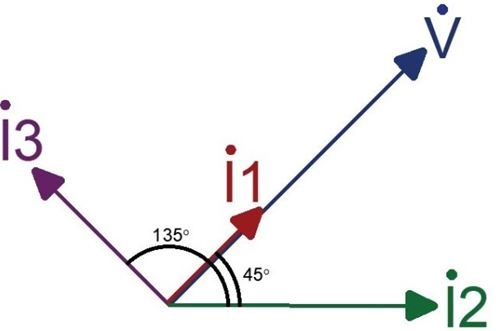
\includegraphics[scale=0.45]{figuras/diagrama.jpg}
    	\label{fig:diagrama}
    	\\
    	\vspace{0.2cm}\hspace{-3cm}\small{Fonte: Silva (2020).}
    \end{figure}
    
    Texto texto texto texto texto texto texto texto texto texto texto texto texto texto texto texto texto texto texto texto texto texto texto texto texto texto texto texto texto texto texto texto, conforme mostra a Equação \ref{eq:baskara}.
    
\begin{equation} \label{eq:baskara}
  x=\frac{-b\pm\sqrt{b^2-4ac}}{2a}
\end{equation} 
